\documentclass[12pt,a4paper,UTF8]{ctexart}
\CTEXsetup[format={\Large\bfseries}]{part}
\CTEXsetup[format={\Large\bfseries}]{section}

\usepackage{ctex}
\usepackage{commath}
\usepackage{gbt7714}
\usepackage{graphicx}
\usepackage{rotating}
\usepackage{hyperref}
\usepackage{booktabs}

% \title{标 题}
% \author{heshiyu}
% \date{\today}


\begin{document}
% \maketitle
\tableofcontents

\part{课程论文题目}
人工智能基本理论及应用研究综述

\part{课程论文内容}
\section{知识表示与推理}
\subsection{知识与知识表示}
\textrm{知识可以理解为事实和与事实相关的规则的集合。与之类似的是离散数学中的命题逻辑的概念,众所周知命题便是各种事实以及事实之间的推断。和命题逻辑一眼样,人工智能领域中的知识也是为了反应事物或者说是事实之间的联系与规则。相较与命题逻辑,此处的知识要求更高一些,我们希望知识至少是相对正确的(相对正确性),希望知识可以用符号等显式的表示出来以便能更好的利用这些知识(可表示、可利用性),当然知识也有很多不确定性。在不同的先决条件或者不同的规则下,所得到的知识也大相径庭。例如生物领域中“橘生淮南则为橘 生于淮北则为枳”,计算机科学中二进制10与十进制的10并不相同。}

\textrm{知识表示不仅在人工智能领域中出现,其还是认知科学领域的重要内容,在AI领域,我们通常希望将知识表示训练的像人一样智慧。}

\begin{enumerate}
    \item AI知识表示:
    \begin{description}
        \item [表示方法] 我们如何表示知识?
        \item [表示范围] 某一表示方法的使用范围?
        \item [表示效果] 某种表示方案的效果如何?
        \item [本身性质] 知识表示本身的性质问题?
    \end{description}
\end{enumerate}

知识表示分为两个步骤,将我们生活中的信息流转化为程序可以识别的信息流,然后模仿人的感知、认知、推理等思维来解决一些人类遇到的费时费力的艰巨任务。

对于AI领域的知识表示,通常有以下方法,见表~\ref{table:知识表示方法应用}。

对于AI中各种知识表示方法的优劣,见表~\ref{table:知识表示方法优劣}。

而另一块是关于确定性推理的概念,即依据我们现有的初始信息或依据,按某种确定的推理策略不断运用库中已有知识来逐步得到确定的结论的推理过程。
而在AI领域,我们的推理是借助程序也叫推理机实现的。

确定性推理的特点见表~\ref{table:qdx特点}:
% Please add the following required packages to your document preamble:
% \usepackage{booktabs}
\begin{table}[htb]
    \centering
    \caption{知识表示方法及应用.}
    \label{table:知识表示方法应用}
    \begin{tabular}{@{}cc@{}}
    \toprule
    知识表示方法               & 应用                                                              \\ \midrule
    一阶谓词逻辑表示法            & 知识表示与推理                                                         \\
    \multicolumn{1}{l}{} &                                                                 \\
    产生式表示法               & \begin{tabular}[c]{@{}c@{}}基于遗传算法的问题求解系统\\ 图搜索求解模型\end{tabular} \\
    \multicolumn{1}{l}{} &                                                                 \\
    框架表示法                & 复杂知识的框架网络                                                       \\
    \multicolumn{1}{l}{} &                                                                 \\
    语义网络表示法              & 机器翻译、问答系统、自然语言理解                                                \\ \bottomrule
    \end{tabular}
\end{table}

\begin{table}[htb]
    \centering
    \caption{各种知识表示方法的优劣.}
    \label{table:知识表示方法优劣}
    \begin{tabular}{@{}ccc@{}}
    \toprule
    知识表示方法               & 优势                                                                           & 劣势                                                                              \\ \midrule
    一阶谓词逻辑表示法            & 自然精确严密易实现                                                                    & \begin{tabular}[c]{@{}c@{}}不能表示不确定的知识\\ 耦合度高,效率低\end{tabular}                   \\
    \multicolumn{1}{l}{} & \multicolumn{1}{l}{}                                                         & \multicolumn{1}{l}{}                                                            \\
    产生式表示法               & \begin{tabular}[c]{@{}c@{}}自然、模块性\\ 有效性、清晰性\end{tabular}                     & \begin{tabular}[c]{@{}c@{}}不能表达具有结构性的知识\\ 效率不高\end{tabular}                     \\
    \multicolumn{1}{l}{} & \multicolumn{1}{l}{}                                                         & \multicolumn{1}{l}{}                                                            \\
    框架表示法                & 结构性、继承性、自然性                                                                  & \begin{tabular}[c]{@{}c@{}}缺乏形式理论\\ 适应能力不强\end{tabular}                         \\
    \multicolumn{1}{l}{} & \multicolumn{1}{l}{}                                                         & \multicolumn{1}{l}{}                                                            \\
    语义网络表示法              & \begin{tabular}[c]{@{}c@{}}强调联系,符合人类思维\\ 描述明确简洁直观\\ 结构化显性描述语义关系\end{tabular} & \begin{tabular}[c]{@{}c@{}}不能保证推论的严格有效\\ 不能处理结点太多的推理\\ 不便表达判断性深层知识\end{tabular} \\ \bottomrule
    \end{tabular}
\end{table}

\subsection{确定性推理}
常见的确定性推理方法有图搜索策略,盲目搜索和启发式搜索等,还有最新的像消解原理
、规则演绎系统以及产生式系统。此处我选择启发式搜索(Heuristic)来介绍他的原理和应用。

\begin{table}[htb]
    \centering
    \caption{确定性推理特点.}
    \label{table:qdx特点}
    \begin{tabular}{@{}cc@{}}
    \toprule
    确定的推理策略、确定的结论                             \\ \hline
    \multicolumn{1}{l}{事实(条件)和知识是构成推理的两个基本要素} \\ \hline
    以数理逻辑的有关理论、方法和技术为理论基础                     \\ \hline
    机械化的、可在计算机上加以实现                           \\ \hline
    \toprule
    \end{tabular}
\end{table}

启发式搜索方法是一种帮你不断试探出答案的方法,但它给出的答案是具有偶然性的,也就是subject to chance。
如在一个状态空间中,对一点的可能所在的每一个位置进行评估,先得到一个最可能的位置。
再从这个位置出发持续进行下一轮的位置评估,这样的循环往复的搜索过程就被称为启发式搜索。
而评估过程所用到的估价函数是启发式搜索核心,可以根据状态场景来选取合适的估价函数,
常见的如式~\ref{eq:启发式搜索估价}:
\begin{equation}
    f(n)=g(n)+h(n)
    \label{eq:启发式搜索估价}
\end{equation}

天气被认为是影响航班路径规划的最主要因素,有70\%的航班延误是由于危险天气\cite{Narkawicz2016}。
Li He和Anfei Zhao\cite{hePathPlanningMethod2019}使用启发式算法将飞机在危险天气下,不同飞行海拔高度对飞机飞行转态的影响离散化进入一个多边网格模型,
结果发现,借助该网格所获得的最小代价的飞行路径比传统的以一个恒定海拔高度飞行的飞行路径要更短。
本章认为,当飞行过程中海拔发生变化,则规划的飞行路径也应适当的变化,详情见图~\ref{fig:path plan change }。
\begin{figure}[htbp]
    \centering
    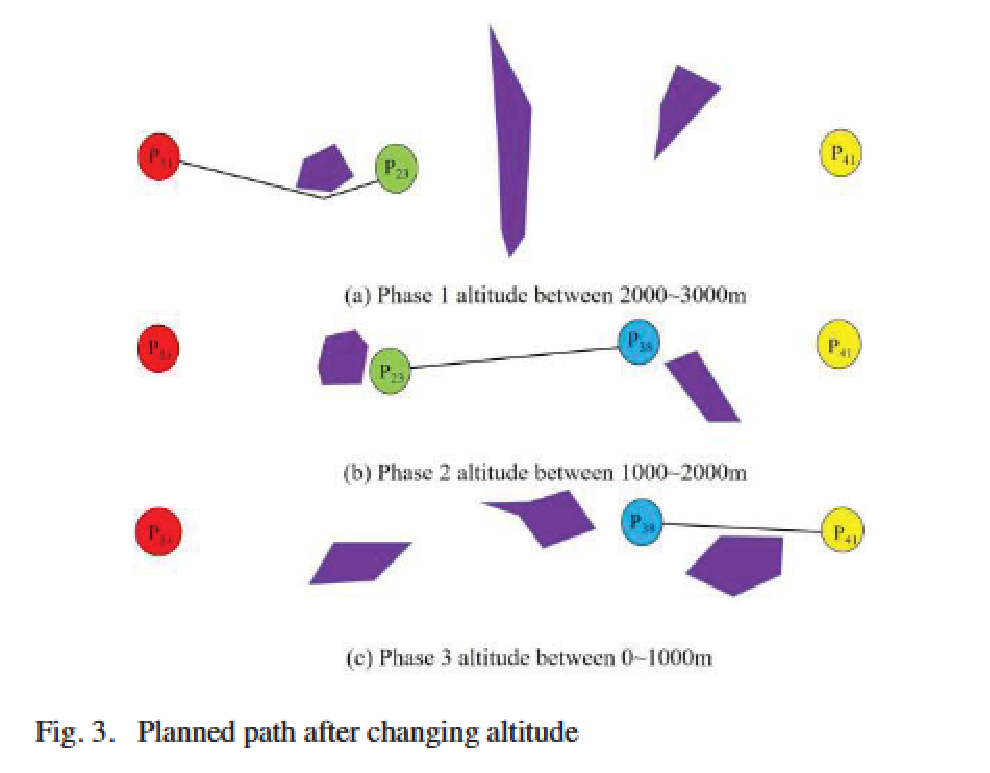
\includegraphics[width=12cm]{allpicture/altitude_change.eps}
    \caption{海拔变化时路径节点变化图.}
    \label{fig:path plan change }
\end{figure}

这篇文章讨论,如果在决策点改变飞行高度,则从决策点到达下一个路径点的成本不是水平面上的欧几里德距离。
因为高度变化被视为在一定爬升角度下的直线飞行,计算到达所选高度后的下一个路径点的代价公式为式~\ref{eq:代价C_height}
\begin{equation}
    C_{\text {height }}=\sqrt{d^2{ }_{\text {height }}+h^2}
    \label{eq:代价C_height}
\end{equation}

$ d_{\text {height }} $是当前决策点与选定高度中的下一个路径点在水平面上的欧几里得距离,$ h $是海拔的变化。
同时,在网格系统中,使用曼哈顿距离作为代价估计的启发式函数具有更好的计算速度和搜索效率\cite{grecheComparisonEuclideanManhattan2017}。
这样做可以确保路径搜索方向始终靠近目标,简化搜索空间,排除远离目标的点。得到的启发式搜索函数中$ h(n) $为~式~\ref{eq:h(n)}。
\begin{equation}
    h(n)=\left|x_g-x_n\right|+\left|y_g-y_n\right|
    \label{eq:h(n)}
\end{equation}
$ n $表示当前网格点,$ g $表示目标点,$ x_g, x_n$等表示相应结点坐标。

则应用次启发式搜索的规划飞行路径的代价函数就为式~\ref{eq:启发式搜索cost函数},$ C_{\text {height }} $表示到达当前结点n之前的代价。
\begin{equation}
    f(n)=C_{\text {height }}+\left|x_g-x_n\right|+\left|y_g-y_n\right|
    \label{eq:启发式搜索cost函数}
\end{equation}

最终的实验结果表明,根据危险天气和海拔的不同,基于启发式搜索的路径决策算法所得到的航班里程要小于恒定海拔下飞行的航班里程。
通过海拔的不断调整,可以将飞机更好的锁定在危险天气影响较小的飞行区域,进而减少平均航行里程\cite{hePathPlanningMethod2019}。

\subsection{不确定性推理}
对比于上文中所讲的确定性推理,不确定性推理便好理解了。
不确定性推理的初始的条件(论据)不确定,推理方法(或策略)也不确定,知识库也不确定,最后的推理结果不确定但合理。
常见的知识不完备、不精确以及模糊知识等的推理也属于不确定推理的范畴。不确定性推理的特点见表~\ref{table:bqdx特点}
\begin{table}[htb]
    \centering
    \caption{不确定性推理特点.}
    \label{table:bqdx特点}
    \begin{tabular}{@{}cc@{}}
    \toprule
    证据的不确定性表示                       \\ \hline
    不确定性的匹配                         \\ \hline
    \multicolumn{1}{l}{组合证据不确定性的计算} \\ \hline
    不确定性的更新                         \\ \hline
    不确定性结论的合成                       \\ \hline
    \toprule
    \end{tabular}
\end{table}

常见的不确定性推理方法有模糊推理、可信度、证据理论、主观贝叶斯方法等等。本文主要选取主观贝叶斯
方法来着重介绍一下。我们都知道贝叶斯公式为式~\ref{eq:bayes},而将全概率公式代入后可得贝叶斯公式的另一种形式,即式~\ref{eq:全概率Bayes}。
\begin{equation}
    P\left(A_i \mid B\right)=\frac{P\left(A_i\right) \times P\left(B \mid A_i\right)}{P(B)}, i=1,2, \ldots, n
    \label{eq:bayes}
\end{equation}

\begin{equation}
    \label{eq:全概率Bayes}
    P\left(A_i \mid B\right)=\frac{P\left(A_i\right) \times P\left(B \mid A_i\right)}{\sum_{j=1}^n P\left(A_j\right) \times P\left(B \mid A_j\right)}
    \end{equation}
引入一组不确定性数值对$ (\mathrm{LS}, \mathrm{LN}) $来表示知识的强度,分别称为充分性度量和必要性度量,即式~\ref{eq:LS}和式~\ref{eq:LN}。
\begin{equation}
    \label{eq:LS}
    L S=\frac{P(E \mid H)}{P(E \mid \neg H)}
\end{equation}
\begin{equation}
    \label{eq:LN}
    L N=\frac{P(\neg E \mid H)}{P(\neg E \mid \neg H)}=\frac{1-P(E \mid H)}{1-P(E \mid-\neg H)}
\end{equation}
则此时得到主观贝叶斯公式为式~\ref{eq:主观Bayes}。
\begin{equation}
    \label{eq:主观Bayes}
    \begin{gathered}
    P(H \mid E)=\frac{P(H) \times P(E \mid H)}{P(E)} \\
    P(\neg H \mid E)=\frac{P(\neg H) \times P(E \mid \neg H)}{P(E)}
    \end{gathered}
\end{equation}
借助几率函数即式~\ref{eq:几率函数}最终可得到分段线插值表示的后验概率为式~\ref{eq:分段Bayes}。
\begin{equation}
    \label{eq:几率函数}
    \begin{gathered}
    O(x)=\frac{P(x)}{1-P(x)}=\frac{P(x)}{P(-x)} \\
    P(x)=\frac{O(x)}{1+O(x)} \\
    P(x)=0 \text { 时, } O(x)=0 \\
    P(x)=1 \text { 时, } O(x)=+\infty
    \end{gathered}
\end{equation}
\begin{equation}
    \label{eq:分段Bayes}
    P(H \mid S)=\left\{\begin{array}{c}
    P(H \mid \neg E)+\frac{P(H)-P(H \mid \neg E)}{P(E)} \times P(E \mid S), 0 \leq P(E \mid S)<P(E) \\
    P(H)+\frac{P(H \mid E)-P(H)}{1-P(E)} \times[P(E \mid S)-P(E)], P(E) \leq P(E \mid S) \leq 1 \\
    \end{array}\right.
\end{equation}

袁杰等\cite{YuanJiYuGaiJinZhuGuanBeiYeSiFangFaShiBieDianRongMeiLuYiChangGongKuang2021}借助改进后的主观贝叶斯方法来
更好的进行电熔镁炉熔炼过程异常工况识别,同时利用模糊隶属度函数对个观测状态和证据进行匹配,对金属熔炼过程中的不确定性问题即异常工况
获取到更好的识别效果。

























\bibliographystyle{gbt7714-numerical}
\bibliography{F:/BibTeXref/zoterorepo.bib}
\end{document}